\chapter{Projekt}
    \section{Wstęp}
    Niniejszy raport prezentuje wyniki prac nad projektem mechanicznego zegara wieżowego.
    W ramach projektu wykonano:
   \begin{itemize}
   	\item model 3D oraz dokumentację płaską w programie NX,
   	\item obliczenia dynamiki mechanizmu zegarowego,
   	\item symulacje wytrzymałościowe najbardziej wytężonych podzespołów.
   \end{itemize}
	
	
        \subsection{Motywacja}
        Powodem podjęcia tego właśnie tematu w ramach przedmiotu Projekt Integrujący, było uświetnienie budynku Instytu Techniki Cieplnej.
        Ponadto dodatkową pobudką była chęć zmierzenia się z nietrywialnym problemem zaprojektowania analogowego zegara o dużych gabarytach.
        Jest to skomplikowany mechanizm, którego sposób działania nie jest zbyt dobrze uokumentowany w powszechnie dostępnej współczesnej literaturze. Takie zegary sa zwykle projektowane w sposób rzemieślniczy. Kolejną motywacją była chęć odkrycia metodologii projektowania takich mechanizmów od strony inżynierskiej.
        \subsection{Przegląd rozwiązań technicznych w technice zegarowej}
        Wśród większości mechanicznych zegarów wieżowych można znaleźć wiele podobieństw.
        Dziełanie najważniejszych cześci może być jednak zreaizowane w różny sposób:
        \begin{enumerate}
        	\item Układ taktujący - istnięją dwa rozwiązania wychwytowe:
        	\begin{itemize}
        		\item symetryczna kotwica wychwytowa - jest zdecydowanie trudniejsza w wykoaniu, wymaga dokładnych tolerancji i bardzo dobrego dopasowania kształtów zębów koła wychwytowego i kotwicy. Jest wykorzystywana w małych dokładnych zegarach.
        		\item niesymetryczna kotwica wychwytowa - jest prostsza w wykonaniu, lecz odmierza czas z mniejszą dokładnością. Jest zwykle wykorzystywana w zegarach wierzowych gdzie dokładnosć co do sekundy nie jest zwykle potrzebna i osiągalna.
        	\end{itemize}
        \item Nie wiem czy coś jeszcze godnego uwagi było
       	\end{enumerate}	

    \section{Założenia projektowe}
    Na początku tworzenia projektu przeanalizowano wiele aspektów całego przedsięwzięcia.
    Miało to na celu stworzyć pierwszy konceptu tego projektu, zdefiniować istotne wielkości dotyczące samej konstrukcji jak i eksploatacji oraz nadać im wstępne wartości.
    W ten sposób powstały wymienione niżej założenia projektowe:
    \begin{itemize}
    	\item Średnica tarczy zegara: 2m. 
    	Wymiar ten dobrano na podstawie obserwacji budynku, na którego szczycie ma się znaleźć zegar.
    	Stwierdzono, że taka średnica pozwoli przechodniom dostrzec wyraźnie pokazywaną przez zegar godzinę.
    	\item Długość wahadła: 4 - 10m.
    	Wybrano taki przedział, ponieważ z jednej strony wahadło ma być widoczne i tym samym pełnić rolę estetyczną konstrukcji.
    	Z drugiej zaś strony nie może być zbyt długie, gdyż rodziłoby to problemy konstrukcyjne.
    	\item Gabaryty mechanizmu: 1x1x1m (z wyłączeniem wahadła).
    	\item Okres drgań pracy wahadła: 4s.
    	Przede wszystkim istotne jest aby była to liczba naturalna, aby w dalszym etapie można było łatwiej dobrać koła zębate przekładni.
    	\item Czas pracy zegara między nakręceniami: 8 dni.
    	Przy określeniu tej wielkości brano pod uwagę możliwe wystąpienie skumulowanych wolnych dni od pracy.
    	
    \end{itemize}

    \section{Podział konstrukcji na moduły}
        \subsection{Układ napędowy - przekładnia mechanizmu}
           \subsubsection{Ciąg główny}
           		Ciąg główny odpowiada łączy magazyn energii z układem taktującym.
           		Układ taktujący naprzemiennie blokuje i pozwala na ruch całego mechanizmu.
           		Kiedy przekładnia jest odblokowana moment siły jest przekazywany przez zestaw przekładni do koła wychwytowego i do wskazówek, połączonych z ciągiem głównym poprzez mechanizm wskazowy.
           		Ciąg główny składa się z 4 kół zębatych o zarysie ewolwentowym, z koła wychwytowego oraz z 4 zębników połączonych z poszczególnymi kołami.
  				Każdy z zębników ma 12 zębów.
  				
  				Układ składa się z następujących elementów (patrz rysunek \ref{fig:kacpermechanizmassmdwg1}):
  				\begin{description}
  					\item[Koło główne] - jest ono połączone z magazynem energii zegara. Posiada ono 96 zębów.
  					\item[Zębnik nr 1] - wspołpracuje z kołem głównym.
  					\item[Koło nr 1] - jest połączone z zębnikiem nr 1. Posiada 72 zęby.
  					\item[Zębnik nr 2] - współpracuje z kołem nr 1.
  					\item[Koło nr 2] - jest połączone z zębnikiem nr 2. Posiada 60 zębów.
  					\item[Zębnik nr 3] - współpracuje z kołem nr 2.
  					\item[Koło nr 3] - jest połączone z zębnikem nr 3. Posiada 30 zębów.
  					\item[Zebnik nr 4] - współpracuje z kołem nr 3.
  					\item[Koło wychwytowe] - jest połączone z zębnikiem nr 4. Posiada 36 niesymetrycznych zębów.
  				\end{description}
  				Razem koła zapewniają przełożenie 600:1.
  				Biorąc pod uwagę, że koło wychwytowe wykonuje 1200 obrotów na jeden dzień pracy (koło ma 36 zębów; mechanizm taktujący pozwala na przesunięcie o jeden ząb na 2 sekundy, czyli pół założonego okresu wahadła) przełożenia zostały dobrane w ten sposób aby otrzymać odpowiednie prędkości obrotowe wskazówek.
  				Koło główne wykonuje 2 obroty w ciągu jednego dnia.
  				\begin{figure}
  					\centering
  					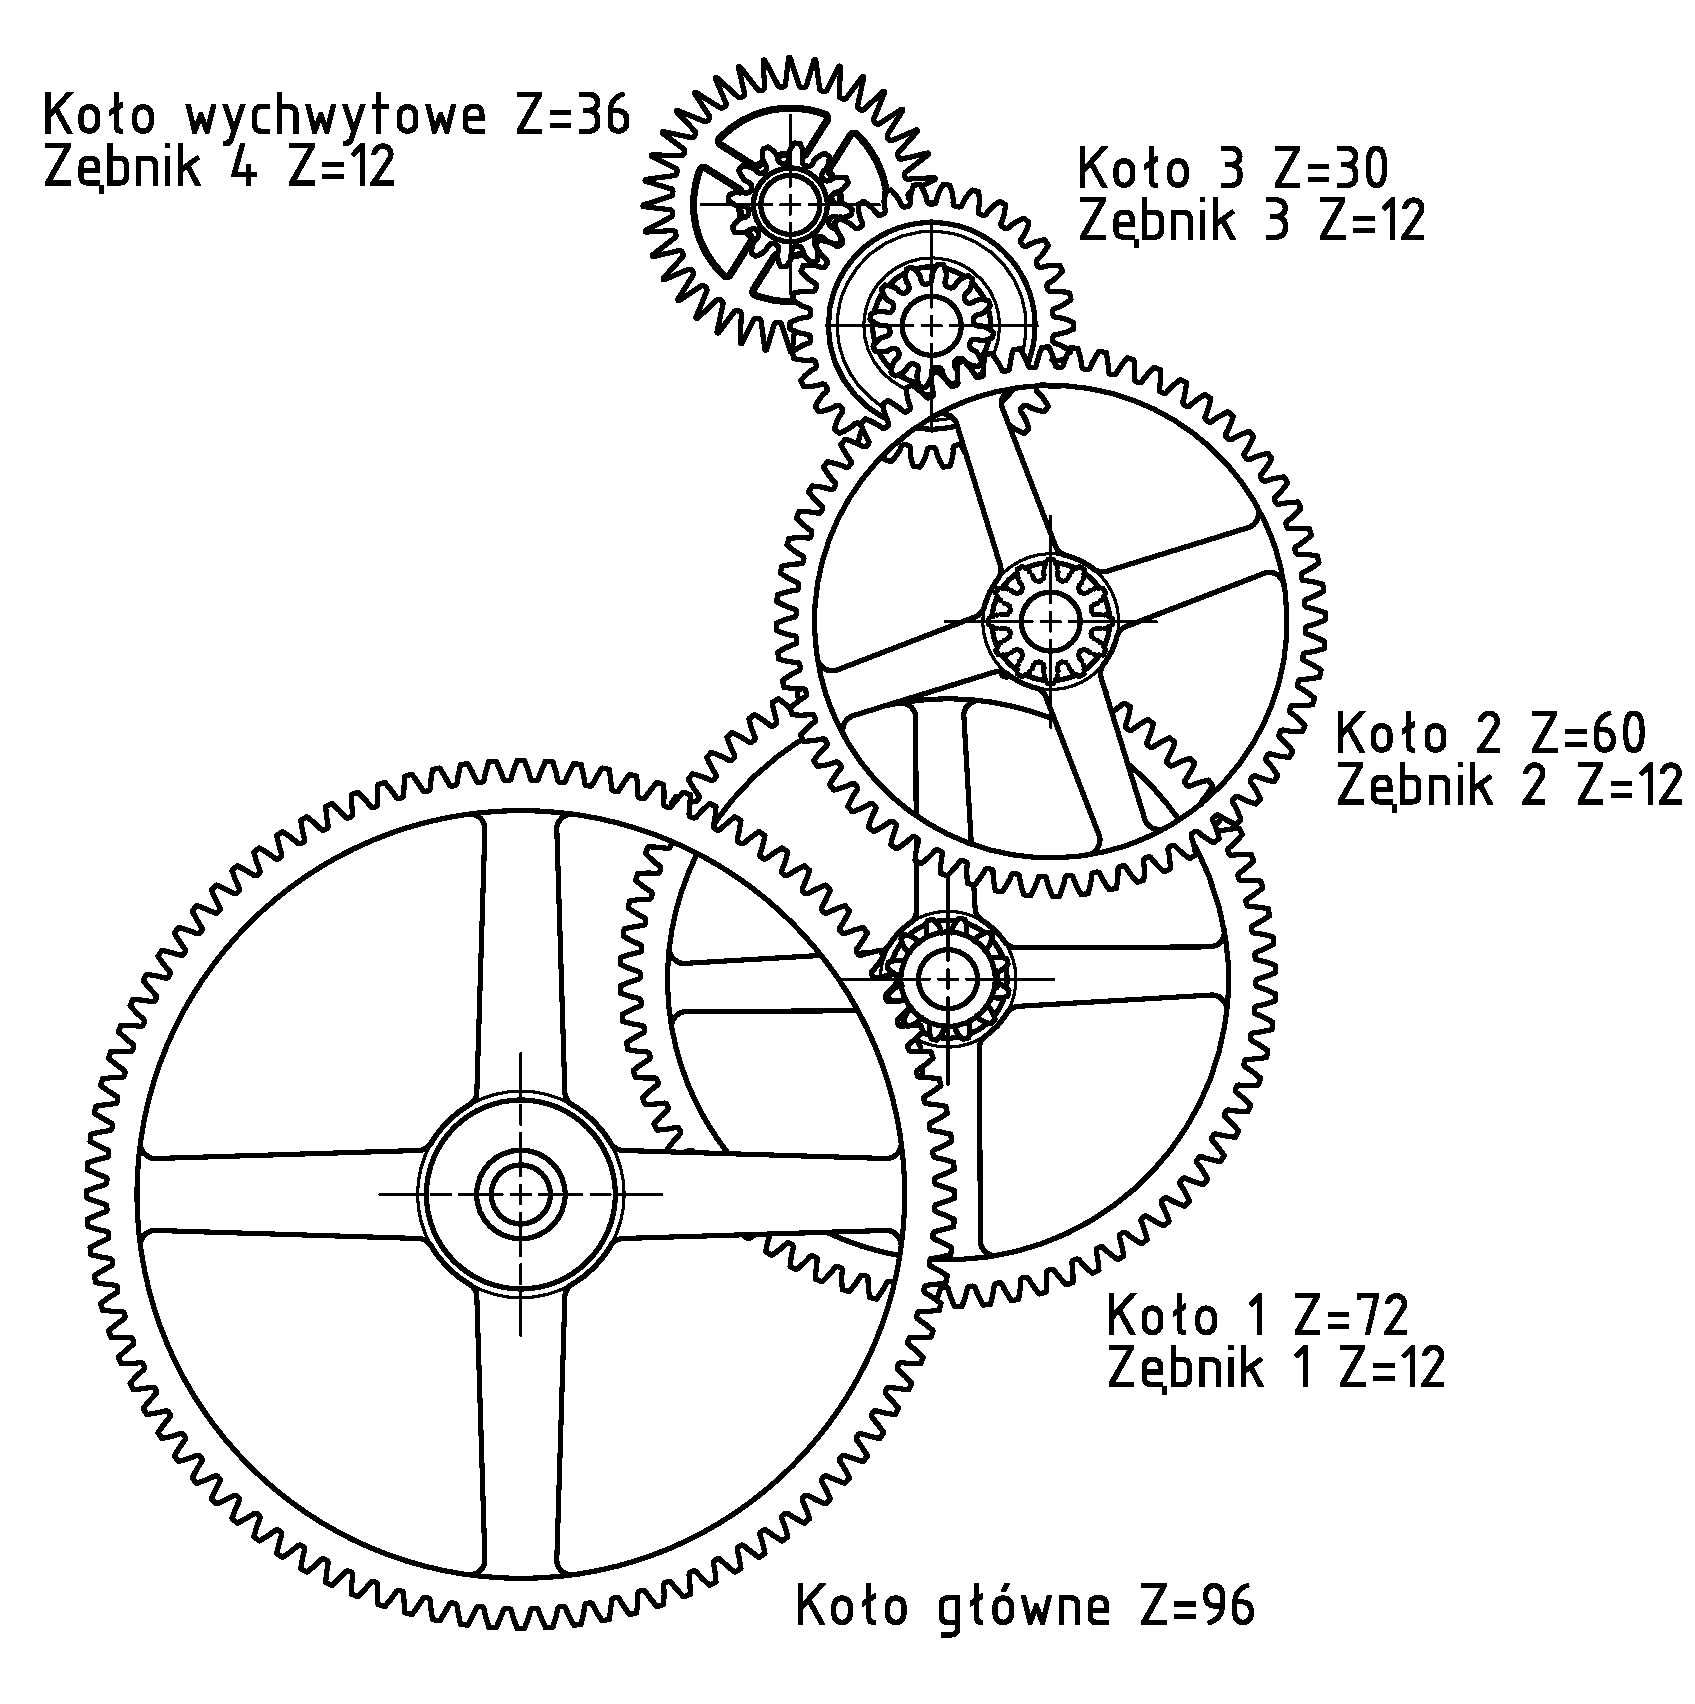
\includegraphics[width=\linewidth]{Projekt/ciag_glowny}
  					\caption{Ciąg główny mechanizmu napędowego.}
  					\label{fig:kacpermechanizmassmdwg1}
  				\end{figure}
  				
  			\subsubsection{Mechanizm wskazowy} 
  				
  				Mechanizm wskazowy składa się z trzech kół zębatych oraz dwóch zębników (patrz rysunek \ref{fig:mechwskaz}):
  				\begin{description}
  					\item[Koło centralne] - współpracuje z kołem nr 1. Posiada 48 zębów.
  					\item[Zebnik nr 5] - jest połączony z kołem centralnym. Posiada 15 zębów.
  					\item[Koło godzinowe nr 1] - współpracuje z zębnikiem nr 5. Posiada 45 zębów. 
  					\item[Zębnik nr 6] - jest połączony z kołem godzinowym nr 1. Posiada 12 zębów.
  					\item[Koło godzinowe nr 2] - współpracuje z zębnikiem nr 6. Posiada 48 zębów. 
  				\end{description} 
  				Koło centralne jest jednocześnie kołem połączonym ze wskazówką minutową. Koła godzinowe zapewniają razem przełożenie 1:12.
  				Dzięki temu wskazówka godzinowa obraca się 2 razy w ciągu jednego dnia.
  				
  				\begin{figure}
  					\centering
  					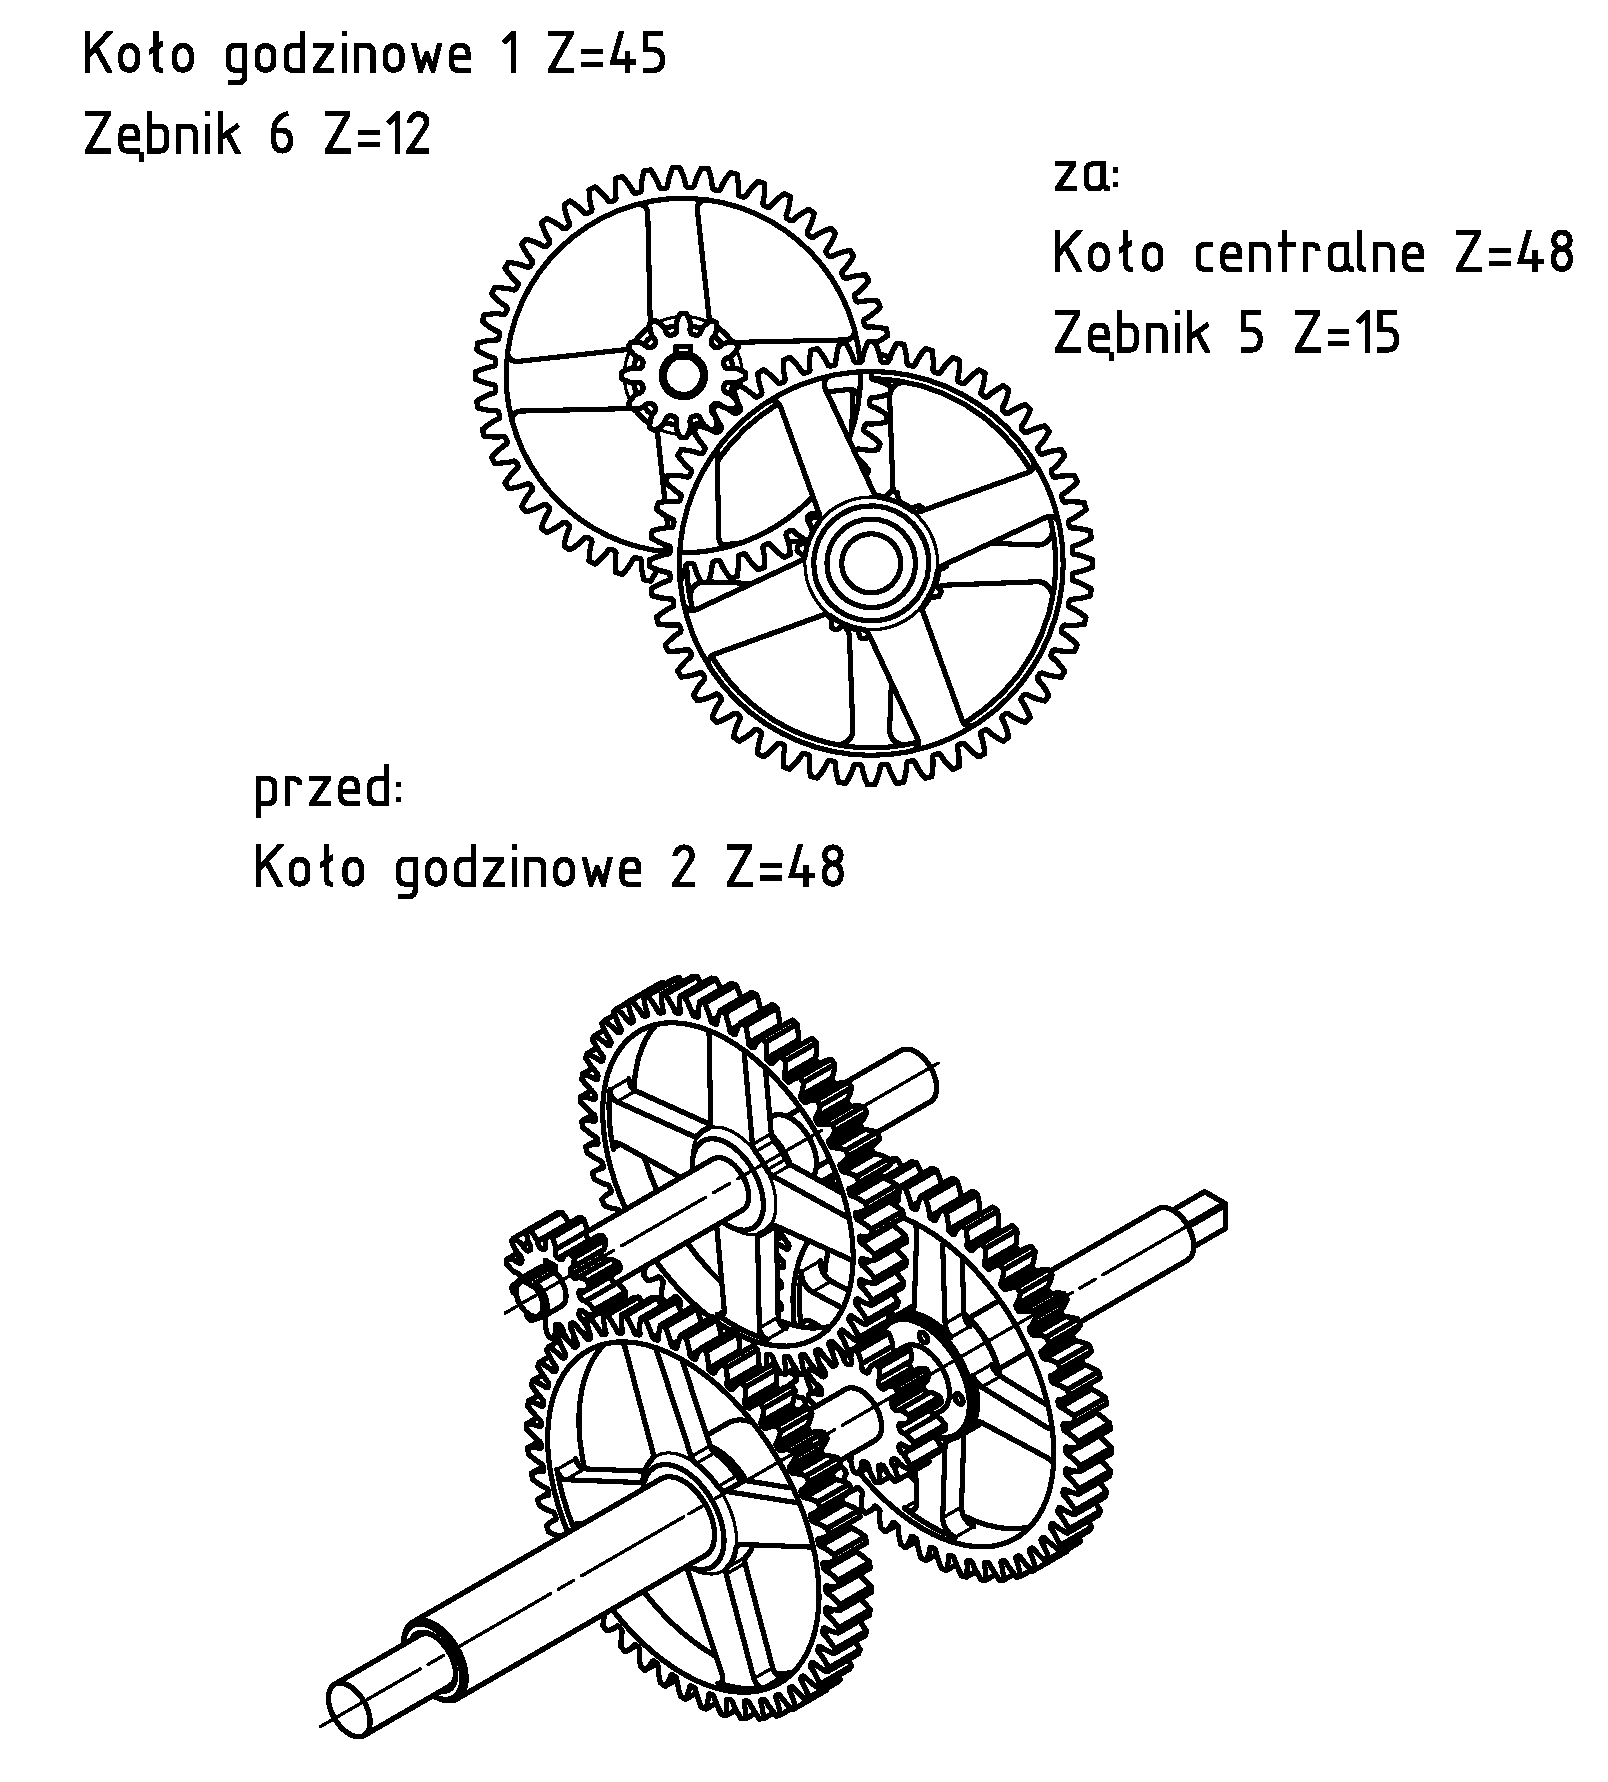
\includegraphics[width=\linewidth]{Projekt/mech_wskaz}
  					\caption{Mechanizm wskazowy}
  					\label{fig:mechwskaz}
  				\end{figure}
  				
        \subsection{Układ napędowy - magazyn energii}
        	Zegar napędzany jest mechanicznie, za pomocą masy na linie nawiniętej na bęben, który jest połączony przez sprzęgło jednokierunkowe z przekładnią. W celu poprawnego działania zegara, napęd musi dysponować wystarczającym momentem, który w każdym takcie dostarczy energię na:

\begin{itemize}
\item Dołożenie energii do wahadła
\item Skompensowanie strat ciernych w przekładni
\item Skompensowanie oporów stawianych wskazówkom przez wiatr oraz ptaki na nich siadające.
\end{itemize}

Powyższe źródła strat stanowią podstawę do budowy modelu energetycznego mechanizmu, na podstawie którego wyznaczono wymiary i masy elementów napędu.

Jako dane wejściowe przyjęto następujące wielkości, przedstawione w tabeli \ref{tab:bebn_zal}:

\begin{table}[h]
\centering
\begin{tabular}{l|c|c|c}
Nazwa & Symbol & Wartość & Jednostka \\ \hline \hline
Czas pracy pomiędzy nawijaniem& \(T_z\) & 8 & dni \\
Okres wahadła & \(T_w\) & 4 & s \\
Prędkość kątowa bębna & \(\omega_b\) & 2 & obr/dzień\\
Przełożenie & \(i_z\) &  600  & - \\
Sprawność przekładni & \(\eta_z\) & 0.8 & - \\
Sprawność wahadła w 1 cyklu & \(\eta_w\) & 0.995 & -\\
Amplituda kątowa wahadła & \(\theta_w\) & 5 & stopnie \\
Moment bezwładności wahadła & \(I_w\) & 1 & \(kg m^2\) \\
Długość bezwładności wahadła & \(L_w\) & 1 & m \\
Masa wahadła & \(m_w\) & 300 & kg \\
\hline
\end{tabular}
\caption{Założenia do pracy zegara. Wszystkie obliczenia prowadzone są w jednostkach SI.}
\label{tab:bebn_zal}
\end{table}


Znając wymiary wahadła można wyznaczyć ilość energii w nim skumulowanej
\begin{equation}
E_w = m_w g  L_w (1-cos(\theta_w))
\end{equation}

Ze sprawności można wyznaczyć stratę energii w jednym cyklu:

\begin{equation}
\Delta E_w = (1-\eta_w)E_w,
\end{equation}

oraz potrzebną ilość energii jaką musi dostarczyć układ napędowy w każdym takcie:

\begin{equation}
\Delta E_b = \frac{\Delta E_w}{\eta_z}.
\end{equation}

Założony czas pracy i częstotliwość pracy wahadła wyznacza ilość potrzebnych cykli:

\begin{equation}
n_z = \lfloor\frac{T_z}{T_w}\rfloor
\end{equation}

Które wyznaczają ilość energii jaką musi wydzielić układ napędowy w jednym okresie pracy (pomiędzy nakręcaniem) \(T_z\):
\begin{equation}
E_b = n_Z \Delta E_b
\end{equation}

Podobnie można wyznaczyć całkowity obrót bębna:
\begin{equation}
\Delta \Theta = \frac{T_z}{\omega_b}
\end{equation}

Parametry swobodne w projekcie bębna to średnica bębna \(D_b\) oraz masa ciężarka \(m_c\). W celu jak najmniejszego obciążenia konstrukcji, Należy tak dobrać te parametry aby moment generowany przez bęben był jak najmniejszy. Można go wyznaczyć bardzo prosto:
\begin{equation}
M_b = \frac{D_b}{2}m_c g
\end{equation}

Jednak dobór nie jest dowolny. Istnieją ograniczenia konstrukcyjne:

Ograniczeniem na średnicę bębna jest maksymalna wysokość o jaką może zostać opuszczony ciężarek - innymi słowy jest to wysokość na której jest zamontowany zegar.

\begin{equation}
\label{eqn:Dbbound}
D_b \leq \frac{\Delta h_{cmax}}{\Delta \Theta_b}
\end{equation}

Zależnie od doboru długości liny i wstępnego nawinięcia, ciężarek może osiąść na ziemi, lub - w przypadku rozwinięcia się całej liny - ramię momentu będzie zerowe. W obydwu przypadkach zegar przestanie pracować, gdyż zatrzymana przekładnia bardzo szybko wytraci energię zmagazynowaną w wahadle.

Ponadto drugie ograniczenie wynika z energii zmagazynowanej w wiszącym ciężarku, które w czasie jednego okresu pracy nie może być mniejsza niż wymagana przez cały mechanizm:
\begin{equation}
\label{eqn:EbBound}
\Delta \Theta_b \frac{D_b}{2} m_c g \geq E_b
\end{equation}

Ostatecznie postawiony jest problem optymalizacji z ograniczeniami. W tym prostym przypadku, można go rozwiązać analitycznie. Ograniczenie \ref{eqn:Dbbound} jest zależne jedynie od średnicy, zatem można zamienić nierówność na równość:

\begin{equation}
D_b = \frac{\Delta h_{cmax}}{\Delta \Theta_b}
\end{equation}

Masa ciężarka jest zatem wyznaczona z ograniczenia \ref{eqn:EbBound}, również poprzez przyjęcie równości:
\begin{equation}
m_c = \frac{2E_b}{g\Delta \Theta_b D_b}
\end{equation}

Takie rozwiązanie daje moment równy:
\begin{equation}
M_b = \frac{E_b}{\Delta \Theta_b}
\end{equation}
Powyższy wzór nie przypadkiem przypomina zależność na pracę którą musi wykonać moment w jednym okresie pracy.

Powyższe wielkości uwzględniają niepewności projektowe, wyrażone przez sprawności przekładni i wahadła. Sprawność przekładni uwzględnia również straty generowane przez wskazówki zegara obciążone warunkami atmosferycznymi i gołębiami siedzącymi na wskazówkach, które wprowadzają moment oporowy. Należyty dobór momentu, bez zbędnego naddatku jest istotny, gdyż wszelkie niespożytkowane zasoby zostaną wydzielone na kole wychwytowym, co będzie prowadzić do szybszego zużycia mechanizmu.

Powyższe wyniki posłużą do dalszych obliczeń, wytrzymałościowych bębna i wahadła.
\begin{figure}
	\centering
	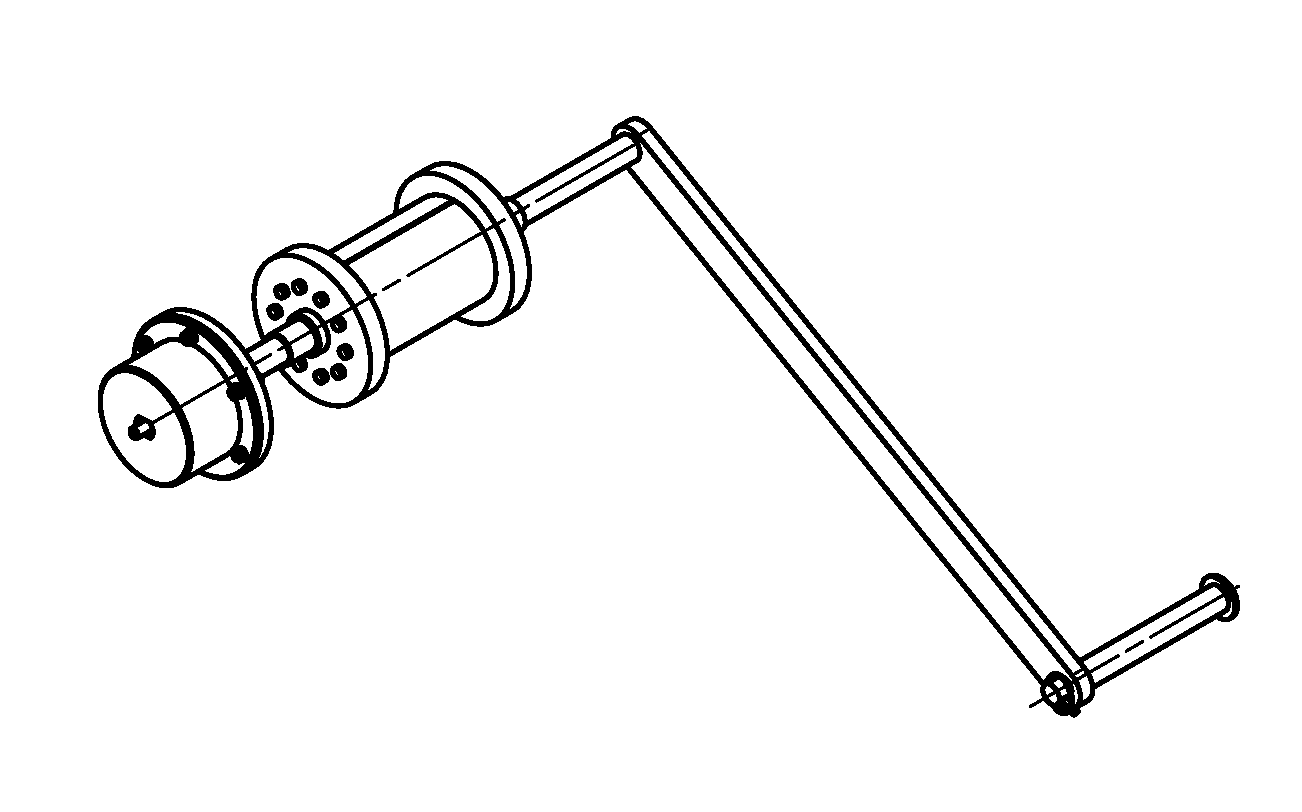
\includegraphics[width=0.9\linewidth]{Projekt/beben}
	\caption{Magazyn energii wahadła - bęben na który nawinięta jest lina z ciężarkiem.}
	\label{fig:beben}
\end{figure}

        \subsection{Wskazówki}
        Kolejnym istotnym elementem projektu są wskazówki.
        Może się wydawać, że istotny jest tylko ich wygląd.
        Jednakże ze względu na obecne w układzie przełożenie, muszą być wystarczająco dobrze wyważone.
        W innym wypadku moment siły wprowadzany z bębna może się okazać nie wystarczający.
        
        \subsection{Układ nastawny}
        Niezbędnym elementem każdego zegara jest moduł pozwalający skorygować wskazywaną godzinę.
        Wiąże się to między innymi ze skończoną dokładnością wykonania wszystkich elementów zegara oraz konieczność zatrzymania go na czas serwisu.
        Analizując możliwe rozwiązania oraz istniejące już konstrukcje, postanowiono zaprojektować ten układ z użyciem sprzęgła.
        Ma ono następujące zalety:
        \begin{itemize}
        	\item Pozwala na dowolny obrót ustawianymi wskazówskami.
        	\item Nie wymaga zatrzymania układu taktującego na czas nastawu godziny.
        \end{itemize}
		Piasta sprzęgła dziala w sposób zaciskowy (patrz rysunek \ref{fig:szpeglo}).
		
		\begin{figure}
			\centering
			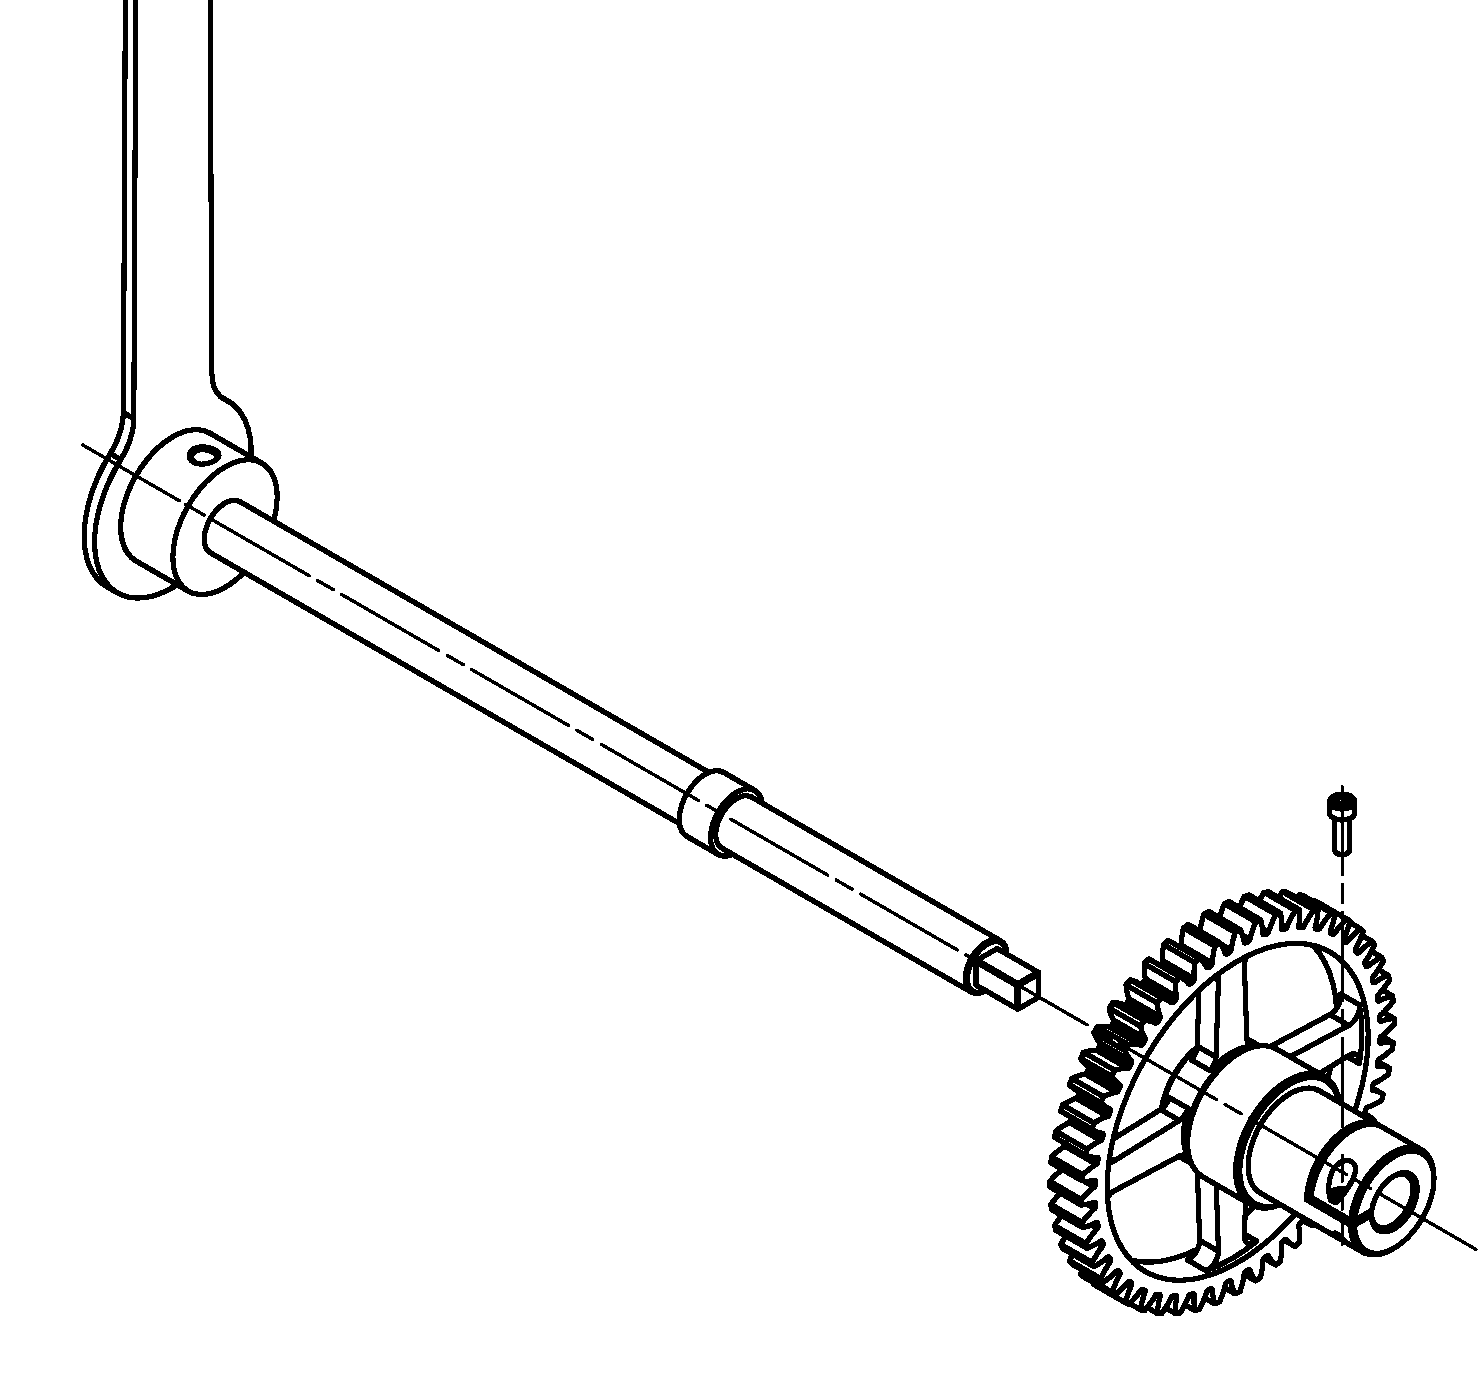
\includegraphics[width=0.8\linewidth]{Projekt/szpeglo}
			\caption{Mechanizmustawiania godziny.}
			\label{fig:szpeglo}
		\end{figure}
		
    	
        \subsection{Układ taktujący}
            Układ taktujący składa się z trzech głównych elementów:
            \begin{itemize}
                \item wahadła;
                \item koła wychwytowego;
                \item wychwytu.
            \end{itemize}
            Okres drgań wahadła fizycznego jest stały. Dzięki temu możliwe jest wykorzystanie wahadła do regulacji czasu jaki zajmuje jeden takt zegara.
            Ruch wahadła jest sprzęgnięty z cała resztą mechanizmu za pomocą koła zębatego nazywanego wychwytowym oraz wychwytu.
            
            Wychwyt jest elementem w kształcie kotwicy (rysunek~\ref{fig::wychwyt}), który naprzemiennie blokuje~i pozwala na swobodny ruch koła wychwytowego.
            Koło jest połączone poprzez przekładnie z całą resztą układu napędowego.
            W ten sposób, gdy koło wychwytowe jest zablokowane, cały mechanizm stoi w miejscu, natomiast gdy może ono się ruszać, moment jest przekazywany przez cały układ napędowy~i wskazówki się przesuwają.

            Ruch wychwytu jest sprzęgnięty z ruchem wahadła. W ten sposób, dobierając odpowiednio ilość zębów koła wychwytowego oraz przełożenia w układzie napędowym, można skorelować długość okresu wahadła z ilością taktów zegara.
            
            \begin{figure}
            \centering
            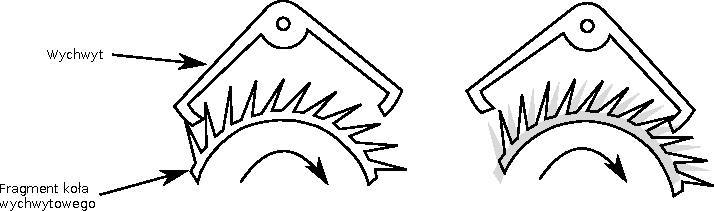
\includegraphics[width=0.9\linewidth]{Obliczenia/wychwyt}
            \caption{Schematyczny rysunek mechanizmu wychwytowego. Na rysunku widoczne są dwa stany w jakich może znajdować się mechanizm. Po lewej stronie zaprezentowana jest sytuacja, w której ruch koła jest zablokowany przez wychwyt po lewej stronie. Po prawej, koło wychwytowe zostało zwolnione, obróciło się (stare położenie jest zaznaczone szarym kolorem), a następnie zostało zablokowane po prawej stronie. Strzałką zaznaczono kierunek obrotu koła wychwytowego.} 
            \label{fig::wychwyt}
            \end{figure}
			
			\begin{figure}
				\centering
				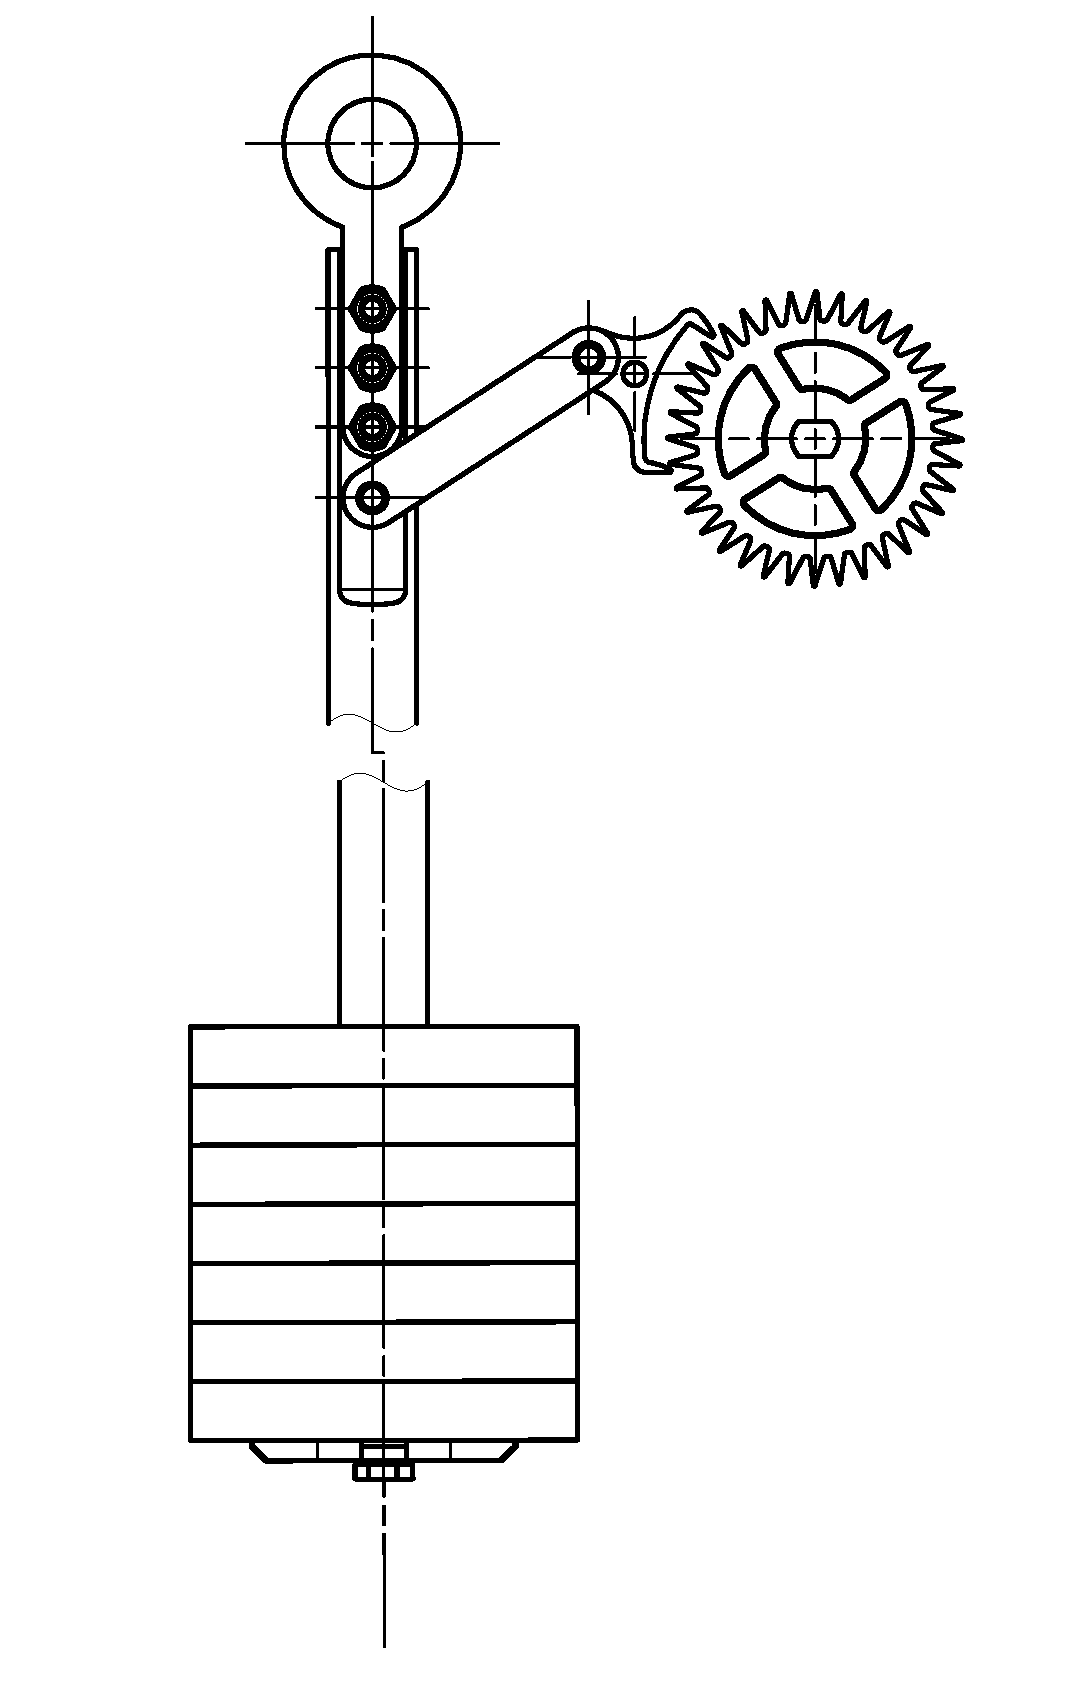
\includegraphics[width=0.6\linewidth]{Projekt/takt}
				\caption{Mechanizm taktujący}
				\label{fig:takt}
			\end{figure}
			

        \subsection{Rama}
        	Rama zostanie wykonana ze spawanych kształtowników stalowych. Podstawowym założeniem było aby była ona niezależna od całej reszty mechanizmu. Wszystkie koła zębate są zamocowane na dwóch stalowych płytach przykręconych do kształtowników. Bęben, na który nawinięta jest lina z ciężarkiem jest ułożyskowany na dwóch łożyskach wahliwych tak, aby kompensować niedokładności ramy wynikające ze spawania.
        	
        	
        \subsection{Projektowe obliczanie wałów}
        	Wszystkie dobrane koła zębate oraz układ dostarczania energii wymagają dobrania wałów o odpowiednich średnicach.
        	W tym celu przeprowadzono obliczenia zginania i skręcania dwóch najbardziej obciążonych wałów: wału do którego przymocowany jest bęben z opuszczający obciążenie oraz wału koła głównego.
        	
        	W przypadku wału z bębnem konieczne jest rozważenie kilku przypadków:
        	\begin{itemize}
        		\item 
        	\end{itemize}
        	\begin{figure}
        		\centering
        		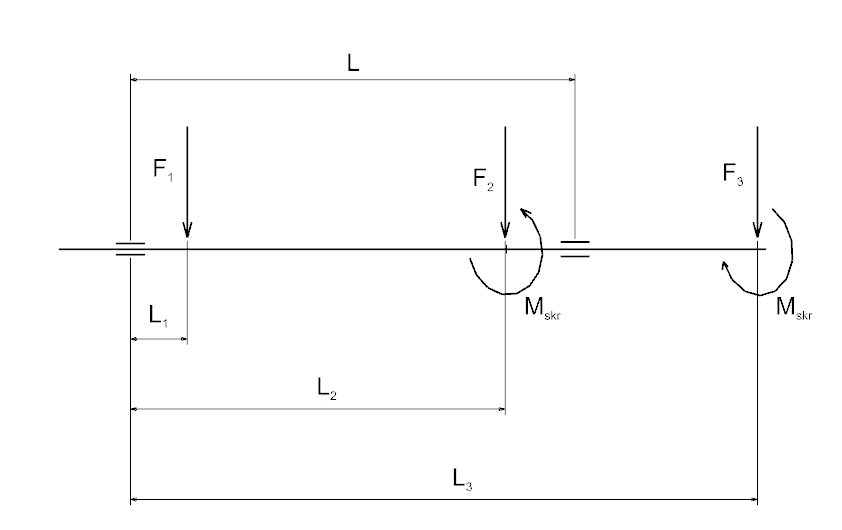
\includegraphics[width=0.9\linewidth]{Projekt/shaft_beben}
        		\caption{Schemat obciążeń przyłożonych do wału, na którym zamocowany jest wolnobieg} 
        		\label{fig::shaft_beben}
        	\end{figure}
        	
        
